\section{Tools} 
Für das Projekt wurden verschiedene Tools für verschiedene Bereiche verwendet. Diese werden nach ihrer Funktion im Folgenden beschrieben.
\subsection*{\textbf{Kommunikation und Meetings}} \label{subsubsec:kommunikation} 
Kommuniziert wurde primär über den webbasierten Instant-Messaging-Dienst Slack. Verschiedene Channels wurden für verschiedene Aufgabenbereiche erstellt, zum Beispiel für die Implementierung, die Präsentationen und für allgemeine Fragen an andere Teammitglieder. Slack wurde teilweise auch für die Kommunikation mit dem Statistance-Team verwendet. Skype wurde als weiteres Kommunikationstool verwendet. Einmal wöchentlich fand ein Meeting über Skype statt. Besonders die Funktion des Screen-Sharings wurde verwendet, um einen Überblick über die Arbeit anderer Teammitglieder zu gewinnen und eine gemeinsame Sicht zu haben. Aufkommende Fragen im Team wurden gesammelt und entweder mit Statistance persönlich besprochen oder in E-Mails an Statistance gesendet. Besonders für die Kommunikation mit Statistance wurden E-Mails geschrieben. Um individuelle Termine für zusätzliche Meetings, Skype Calls und Rücksprachen mit Statistance zu vereinbaren wurden Umfragen über doodle gemacht. So konnten Termine zeitnahe gefunden werden. Meetings mit Statistance wurden anschließend über E-Mail Kontakt mit dem Unternehmen kommuniziert.

\subsection*{\textbf{Sprint-Planung}}
Für den Sprint-Überblick und den Status der dem Sprint zugeordneten Aufgaben wurde ein Trello-Board verwendet. Die Aufgaben konnten zunächst gesammelt und dann bestimmten Teammitgliedern zugewiesen werden. Durch die verschiedenen Zustände in Progress, Review und Done konnten Teammitglieder den Bearbeitungsstand der eigenen Aufgaben dokumentieren und den von Aufgaben andere Mitglieder gut nachvollziehen. Zudem konnten Informationen beispielsweise zum Setup für andere Teammitglieder festgehalten werden. Ein Zwischenstand vom Trello Board ist in \ref{fig:trello} zu sehen.

\begin{figure}[!h]
\centering
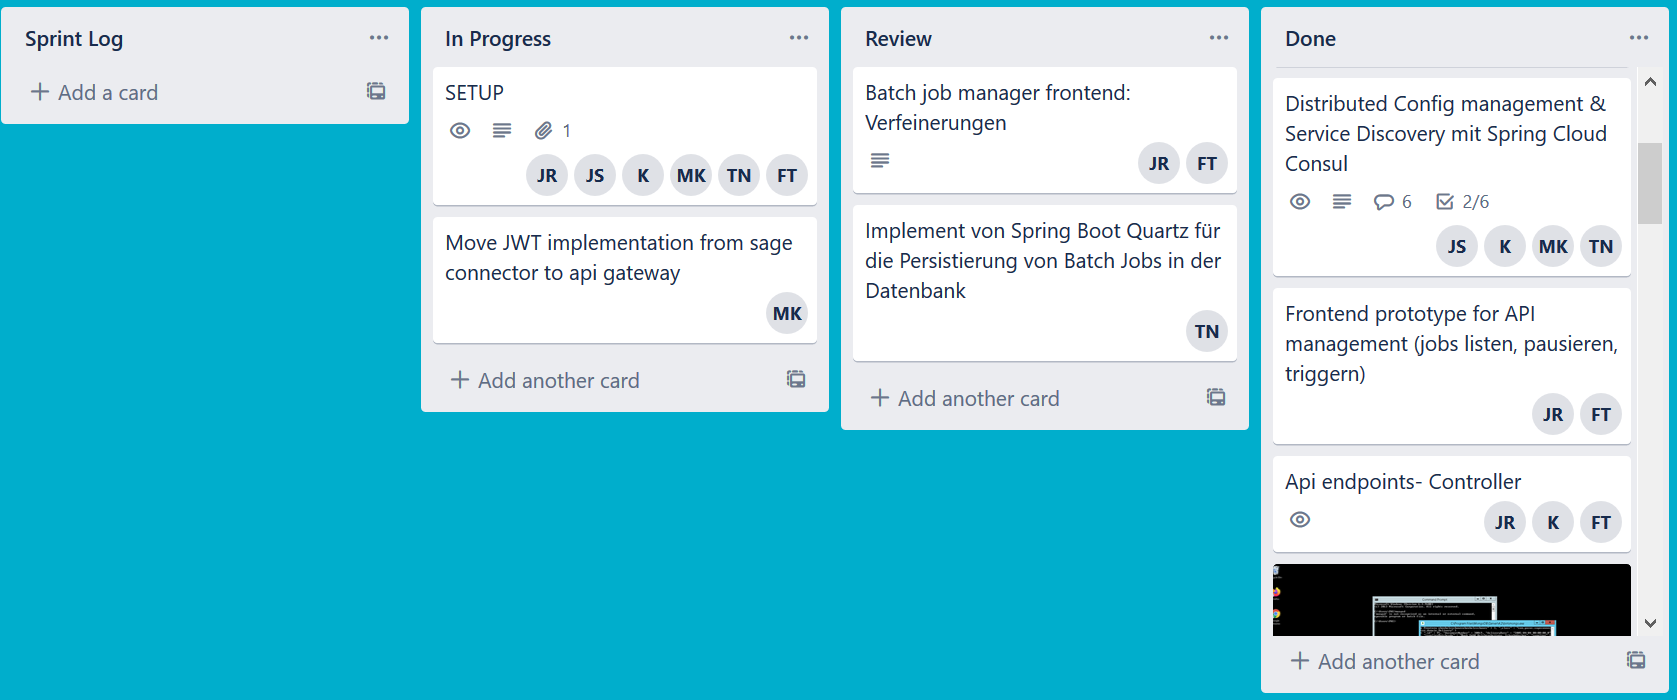
\includegraphics[width=15cm]{images/0x_organization/TrelloBoard.PNG}
\caption{Trello Board}
\label{fig:trello}
\end{figure}

\subsection*{\textbf{Implementierung}}
Für die gemeinsame Implementierung wurden Repositories in gitlab verwendet. Ein Vorteil den die Webanwendung gitlab bietet ist die Versionsverwaltung von Softwareprojekten. Durch die Implementierung in verschiedenen Branches konnten einzelne Aufgaben voneinander getrennt bearbeitet werden und abschließend in den Master Branch gepusht werden. Die einzelnen Arbeiten der Teammitglieder konnten über diesen Weg nicht nur geteilt, sondern auch nachvollzogen werden.

\subsection*{\textbf{Dokumentation}}
Um mit Statistance insbesondere die Rechercheergebnisse zu teilen, wurde Google Drive verwendet. In einem Studenten-Bereich von Statistance konnten alle Dokumente zur Recherche, wie zum Beispiel zu einzelnen Frameworks, Statistance zur Verfügung gestellt werden. Zur fortlaufenden Dokumentation von Meetings und Rücksprachen mit Statistance wurde ein Team Dokument in Google docs verwendet. Hier wurden von Projektstart bis Projektende jegliche Festlegungen, Treffen und sonstige wichtige Informationen festgehalten. Für den Abschlussbericht wurde Overleaf zur gemeinsamen Bearbeitung verwendet.


